\documentclass[../main.tex]{subfiles}
\graphicspath{{\subfix{../figures/}}}

\begin{document}
\section{UML概述}
UML(Unified Modeling Language),全称为\textbf{统一建模语言}:是一种通用的可视化建模语言,用于说明、可视化、构造并文档化软件系统。

模型是对事物的一种抽象,人们常常在正式建造实物之前,首先建立一个简化的模型,以便更透彻地了解它的本质,抓住问题的要害;
在模型中,人们总是剔除那些与问题无关的、非本质的东西,从而使模型与真实的实体相比更加简单、易于把握;
\textbf{模型}:在软件开发期间所产生的中间描述或文档。
\begin{figure}[H]
  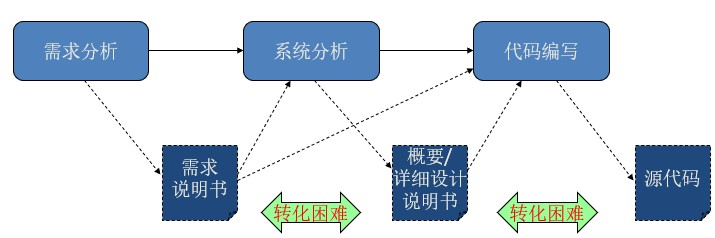
\includegraphics[width=0.70\textwidth]{2_1.jpg}
\end{figure}
构造软件模型通常出于以下几个目地:
\begin{itemize}
  \item 对复杂问题进行简化;
  \item 用于同客户或其他相关人员进行交流;
  \item 加强视觉效果;
  \item 在着手解决一个复杂问题之前,对解决方案进行检测。
\end{itemize}
\begin{enumerate}
  \item 八十年代至九十年代,出现了数量众多的面向对象建模语言.
  \item 1996年,由Grady Booch、Dr.Ivar Jacobson和Dr.James Rumbaugh三人正式推出UML.
  \item UML为人们提供了从不同的角度去观察和展示系统的各种特征的一种标准表达方式。
  \item UML中,从任何一个角度对系统所作的抽象都可能需要用几种模型图来描述,而这些来自不同角度的模型图最终组成了系统的完整模型。
\end{enumerate}
一般而言,可从以下几种常用视角来描述一个系统:
\begin{enumerate}
  \item \textbf{系统的使用实例}:从系统外部的操作者的角度描述系统的功能。
  \item \textbf{系统的逻辑结构}:描述系统内部的静态结构和动态行为,即从内部描述如何设计实现系统功能。
  \item \textbf{系统的物理构成}:描述系统由哪些程序构件所组成。
  \item \textbf{系统的并发性}:描述系统的并发性,强调并发系统中存在的各种通信和同步问题。
  \item \textbf{系统的配置}:描述系统的软件和各种硬件设备之间的配置关系。
\end{enumerate}
\textbf{UML的主要构成}:
\begin{enumerate}
  \item \textbf{视图(views)}:从一个特殊的角度观察到的系统称为一个视图。
    视图由多个图(Diagrams)构成,它不是一个具体的图,而是在某一个抽象层上,对系统的抽象表示。
  \item \textbf{图(Diagrams)}
  \item \textbf{模型元素(Model elements)}:代表面向对象中的类,对象,关系和消息等概念,是构成图的最基本的常用的元素。一个模型元素可以用于多个不同的图中。分为以下两类:
    \begin{itemize}
      \item \textbf{基元素}:是已由UML定义的模型元素。如:类、结点、构件、注释、关联、依赖和泛化等。
      \item \textbf{构造型元素}:在基元素的基础上增加了新的定义而构造的新的模型元素。如扩展基元素的语义(不能扩展语法结构)。
        构造型元素用括在双尖括号``<< >>''中的字符串表示。
    \end{itemize}
  \item \textbf{通用机制(general mechanism))}
\end{enumerate}
\textbf{视图}:
\begin{itemize}
  \item Use case View(Use case 视图):描述系统的外部特性、系统功能等。
  \item Design View(设计视图):描述系统设计特征,包括结构模型视图和行为模型视图,前者描述系统的静态结构(类图、对象图),后者描述系统的动态行为(交互图、状态图、活动图)。
  \item Process View(过程视图):表示系统内部的控制机制。常用活动图描述过程结构,用交互图描述过程行为。
  \item Implementation View(实现视图):表示系统的实现特征,常用构件图表示。
  \item Deployment View(配置视图):配置视图描述系统的物理配置特征。用配置图表示。
\end{itemize}
\textbf{图}:
UML主要提供了\textbf{五类十种}图形:
\begin{itemize}
  \item \textbf{用例图}(Use case diagram):从用户角度描述系统功能,并指出各功能的操作者。
  \item 静态图(Static diagram):表示系统的静态结构,包括\textbf{类图、对象图、包图}。
    \begin{itemize}
      \item 类图描述系统中类的静态结构。不仅定义系统中的类,表示类之间的联系如关联、依赖、聚合等,也包括类的内部结构(类的属性和操作)
      \item 对象图是类图的实例,几乎使用与类图完全相同的标识。他们的不同点在于对象图显示类的多个对象实例,而不是实际的类。
      \item 包由包或类组成,表示包与包之间的关系。包图用于描述系统的分层结构。UML
        1.1 不再认为包图是一类独立的图形.
    \end{itemize}
  \item 行为图(Behavior diagram):描述系统的动态行为。包括\textbf{状态图、活动图}。
    \begin{itemize}
      \item 状态图描述类的对象所有可能的状态以及事件发生时状态的转移条件。通常,状态图是对类图的补充。
      \item 活动图描述满足用例要求所要进行的活动以及活动间的约束关系,有利于识别并行活动。
    \end{itemize}
  \item 交互图(Interactive diagram):描述对象间的交互关系。包括\textbf{顺序图、合作图(通信图)}。
    \begin{itemize}
      \item 顺序图显示对象之间的动态合作关系,它强调对象之间消息发送的顺序,同时显示对象之间的交互;
      \item 合作图描述对象间的协作关系,合作图跟顺序图相似,显示对象间的动态合作关系。
      \item UML 2.0中新增时间图、交互概述图。
    \end{itemize}
  \item 实现图(Implementation diagram):用于描述系统的物理实现,包括\textbf{构件图、配置图}。
    \begin{enumerate}
      \item 构件图描述代码部件的物理结构及各部件之间的依赖关系。
      \item 配置图定义系统中软硬件的物理体系结构。它可以显示实际的计算机和设备(用节点表示)以及它们之间的连接关系,也可显示连接的类型及部件之间的依赖性。
    \end{enumerate}
\end{itemize}
\begin{figure}[H]
  \begin{minipage}{0.5\linewidth}
    \centering
    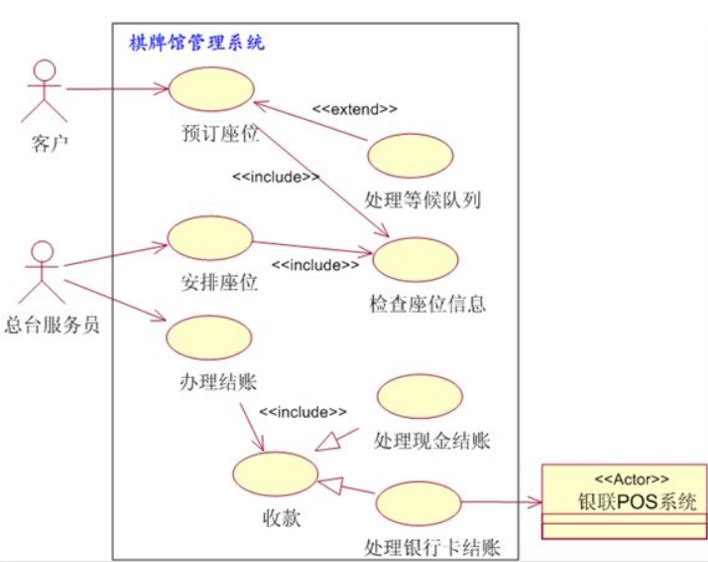
\includegraphics[scale=0.5]{2_2.jpg}
    \caption{用例图}
  \end{minipage}
  \begin{minipage}{0.5\linewidth}
    \centering
    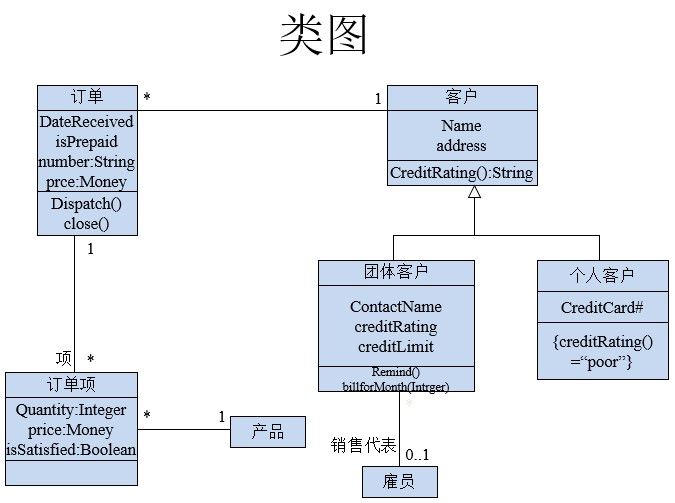
\includegraphics[scale=0.5]{2_4.jpg}
    \caption{类图}
  \end{minipage}
\end{figure}
\begin{figure}[H]
  \begin{minipage}{0.5\linewidth}
    \centering
    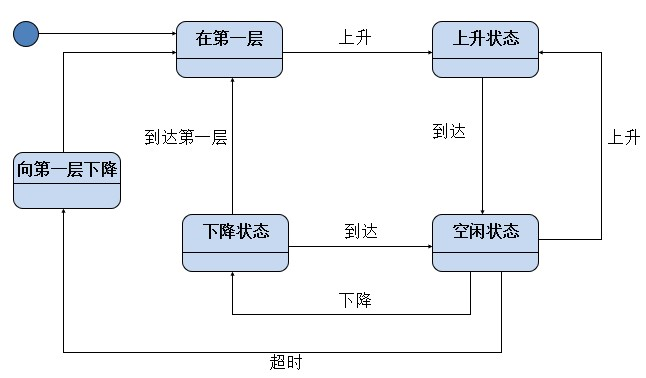
\includegraphics[scale=0.5]{2_5.jpg}
    \caption{状态图}
  \end{minipage}
  \begin{minipage}{0.5\linewidth}
    \centering
    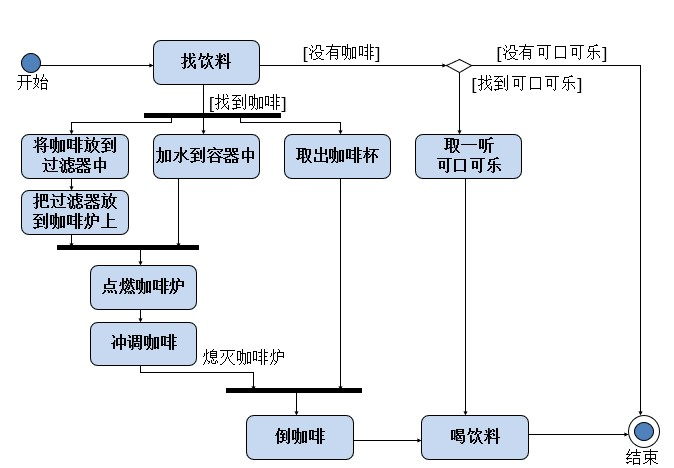
\includegraphics[scale=0.5]{2_6.jpg}
    \caption{活动图}
  \end{minipage}
\end{figure}
\begin{figure}[H]
  \begin{minipage}{0.5\linewidth}
    \centering
    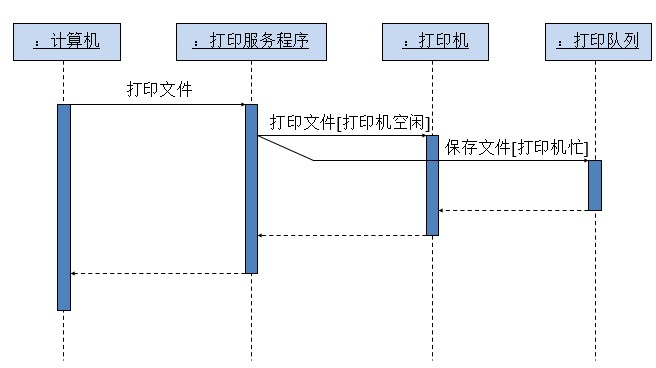
\includegraphics[scale=0.5]{2_7.jpg}
    \caption{顺序图}
  \end{minipage}
  \begin{minipage}{0.5\linewidth}
    \centering
    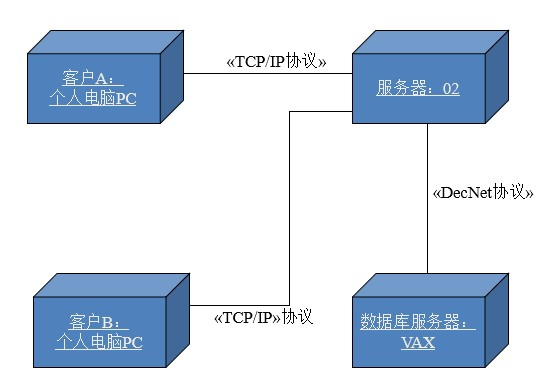
\includegraphics[scale=0.5]{2_8.jpg}
    \caption{配置图}
  \end{minipage}
\end{figure}
\textbf{UML的应用领域}:UML的目标是以面向对象图的方式来描述任何类型的系统,具有广泛的应用领域。其中最常用的是建立软件系统的模型,但它同样可以用于描述非软件领域的系统,如机械系统、企业机构或业务过程,以及具有实时要求的工业系统或工业过程等。
UML可应用于软件开发的各个阶段.\\
\textbf{常用的模型元素}:
\begin{figure}[H]
  \centering
  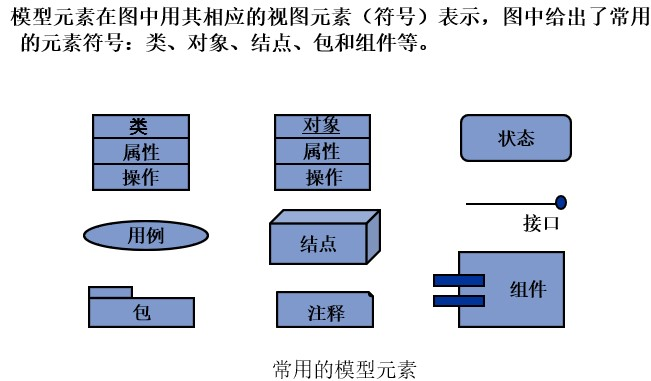
\includegraphics[width=0.7\textwidth]{2_3.jpg}
\end{figure}
\begin{figure}[H]
  \centering
  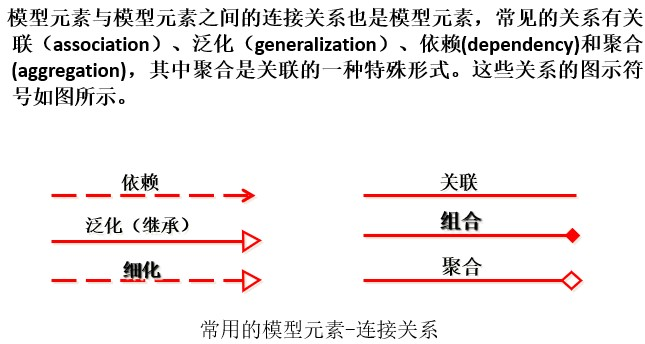
\includegraphics[width=0.7\textwidth]{2_9.jpg}
\end{figure}
\end{document}
